\documentclass[border=1cm]{standalone}
\usepackage{tikz}
\begin{document}

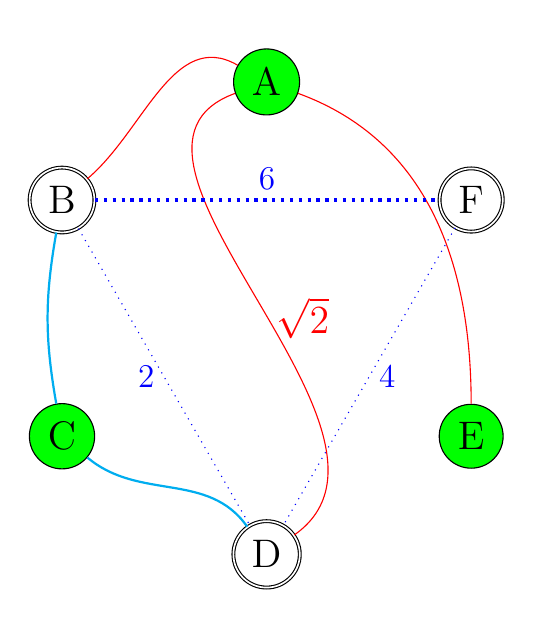
\begin{tikzpicture}
    % Определение узлов в цикле
    \foreach \angle/\label/\col in {150/B/white, 270/D/white, 30/F/white} {
        \node[circle, draw, double, fill=\col, minimum size=0.8cm] (\label) at (\angle:3cm) {\Large \label};
    }
    \foreach \angle/\label/\col in {90/A/green, 210/C/green, 330/E/green} {
        \node[circle, draw, fill=\col, minimum size=0.8cm] (\label) at (\angle:3cm) {\Large \label};
    }
    
    % Соединения
    \draw[red] (A) to[out=150, in=40] (B);
    \draw[red] (A) to[out=200, in=35] (D) node[midway, right] {\Large $\sqrt{2}$}; % Кривая sqrt(2)
    \draw[red] (A) to[out=340, in=90] (E);
    
    \draw[blue, dotted, very thick] (B) -- (F) node[midway, above] {\large 6};
    \draw[cyan, thick] (B) to[out=260, in=100] (C);
    
    \draw[blue, dotted] (B) -- (D) node[midway, left] {\large 2};
    \draw[blue, dotted] (F) -- (D) node[midway, right] {\large 4};
    \draw[cyan, thick] (C) to[out=320, in=125] (D);

\end{tikzpicture}

\end{document}